\chapter{플랫폼과 조세}\label{cha:taxation}

\section*{학습개요}
플랫폼 경제 더 폭넓게는 디지털 경제에서의 조세 문제를 학습한다.


\section*{학습목표}
\begin{enumerate}
\item 디지털 경제와 플랫폼 사업의 특징을 설명할 수 있다.
\item 디지털 경제와 플랫폼 사업이 전통적인 조세 체계를 어떤 방법으로 우회하는 지 이해한다.
\item 2021년 합의된 국제 디지털세 도입의 방향을 설명할 수 있다.
\end{enumerate}

\section*{주요 용어}
고정사업장 소재지국의 과세권 행사, 정상거래원칙에 근거한 무형 자산 과세, 국제 디지털 세

\pagebreak

\section{전통적인 조세 체계의 한계}\label{sec:}
\begin{itemize}
\item 디지털 경제의 사업 유형 분류 \citep{Hagiu:2015wg}
	\begin{itemize}
	\item 다면 플랫폼(multi-sided platform)
		\begin{itemize}
		\item 플랫폼을 통해 각 면의 사용자가 거래
		\item 간접 네트워크 효과가 중요
		\item[예)] 구글, 에어비앤비, 페이스북 등
		\end{itemize} 
	\item 재판매(resellers)
		\begin{itemize}
		\item 공급자로부터 상품을 구매하여 소비자에게 재판매
		\item 재판매자가 플랫폼이어야할 필요는 없으며, 최종 사용자(공급자와 소비자) 간의 상호 작용은 없음
		\item[예)] 아마존 전자 상거래, 애플 뮤직, 스포티파이, 넷플릭스 (영상을 구매하여 배급하는 경우) 등
		\end{itemize}
	\item 수직 통합(vertically integrated firms)
		\begin{itemize}
		\item 공급자 또는 그 역할을 계열사로 합병하거나, 그 역할을 맡고 있는 경우
		\item[예)] 아마존 물류, 넷플릭스 (영상 제작 및 투자) 등
		\end{itemize}
	\item 중간재 공급(input suppliers)
		\begin{itemize}
		\item 다른 기업의 상품이나 서비스 생산 과정에 필요한 중간재를 공급
		\item 최종 소비자와 거래할 필요가 없음
		\item[예)] 게임 엔진 개발사 등
		\end{itemize}
	\end{itemize}
\item 플랫폼 사업과 디지털화의 특징\footnote{이후에서는 플랫폼 산업의 특성으로 인한 것, 디지털화로 인한 것을 엄격히 구분하지는 않았음} \cite[ch. 2]{OECD/G20-Base-Erosion-and-Profit-Shifting-Project:2018to}
	\begin{itemize}
	\item 소득의 원천이 되는 국가에 물리적 고정 사업장을 두지 않고, 사법 경계를 가로질러 대단위 경제 활동이 가능 \footnote{다국적 기업을 생각해보면, 디지털 플랫폼 사업자의 고유한 특성은 아님}
	\item 소프트웨어와 알고리듬 등 지적재산권을 포함한 무형 자산에 크게 의존\footnote{지적재산권이 중요한 수입원이 되는 것 또한 디지털 플랫폼 사업자의 고유한 특성은 아님}
	\item 데이터, 사용자 참여 등은 지적재산권과 함께 시너지(synergy) 효과를 냄 $\rightarrow$ 부가가치를 만드는 주체가 사용자가 됨\footnote{사용자 참여를 서비스 사용에 대한 대가로 보는 입장도 있음. 이러한 입장에서는 사용자가 생산한 데이터에 대해 소득세 부과가 가능하다고 주장하게 됨. 물론 수동적인 소비자가 다수일 수 있다는 점 그리고 화폐로 환산하기로 어려운 소비자 참여가 있다는 점도 있음}
	\end{itemize}	
\item 전통적인 조세 체계를 위협
	\begin{itemize}
	\item 고정사업장(permanent establishment) 소재지국의 과세권 행사
		\begin{itemize}
		\item $\rightarrow$ 전세계에서 발생하는 소득에 대해 기업의 본사 소재지국에서만 과세권 행사 가능
			\begin{itemize}
			\item $\rightarrow$ 해당 상품을 소비하는 소비자가 소재하는 국가 입장에서는 재정 위협\footnote{고정사업장 유무에 관계없이 해당 기업의 판매가 이루어지는 시점의 소비자 소재지 국가에서 과세권을 가질 수도 있음. 그러나 이를 일반적으로 인정하는 경우, 국제적인 이중 과세 발생 가능성이 높고 이로 인해 기업의 세 부담 및 납세 협력 비용이 높아짐에 따라, OECD 모델조세조약이나 UN 모델 조세조약 또는 국가별 조세 조약 체결 시, 고정사업장이 있어야만 소비 원천지 국가에서 과세할 수 있는 것으로 규정하는 것이 일반적}
			\end{itemize}
			
				\begin{figure}[htbp]
				\begin{center}
				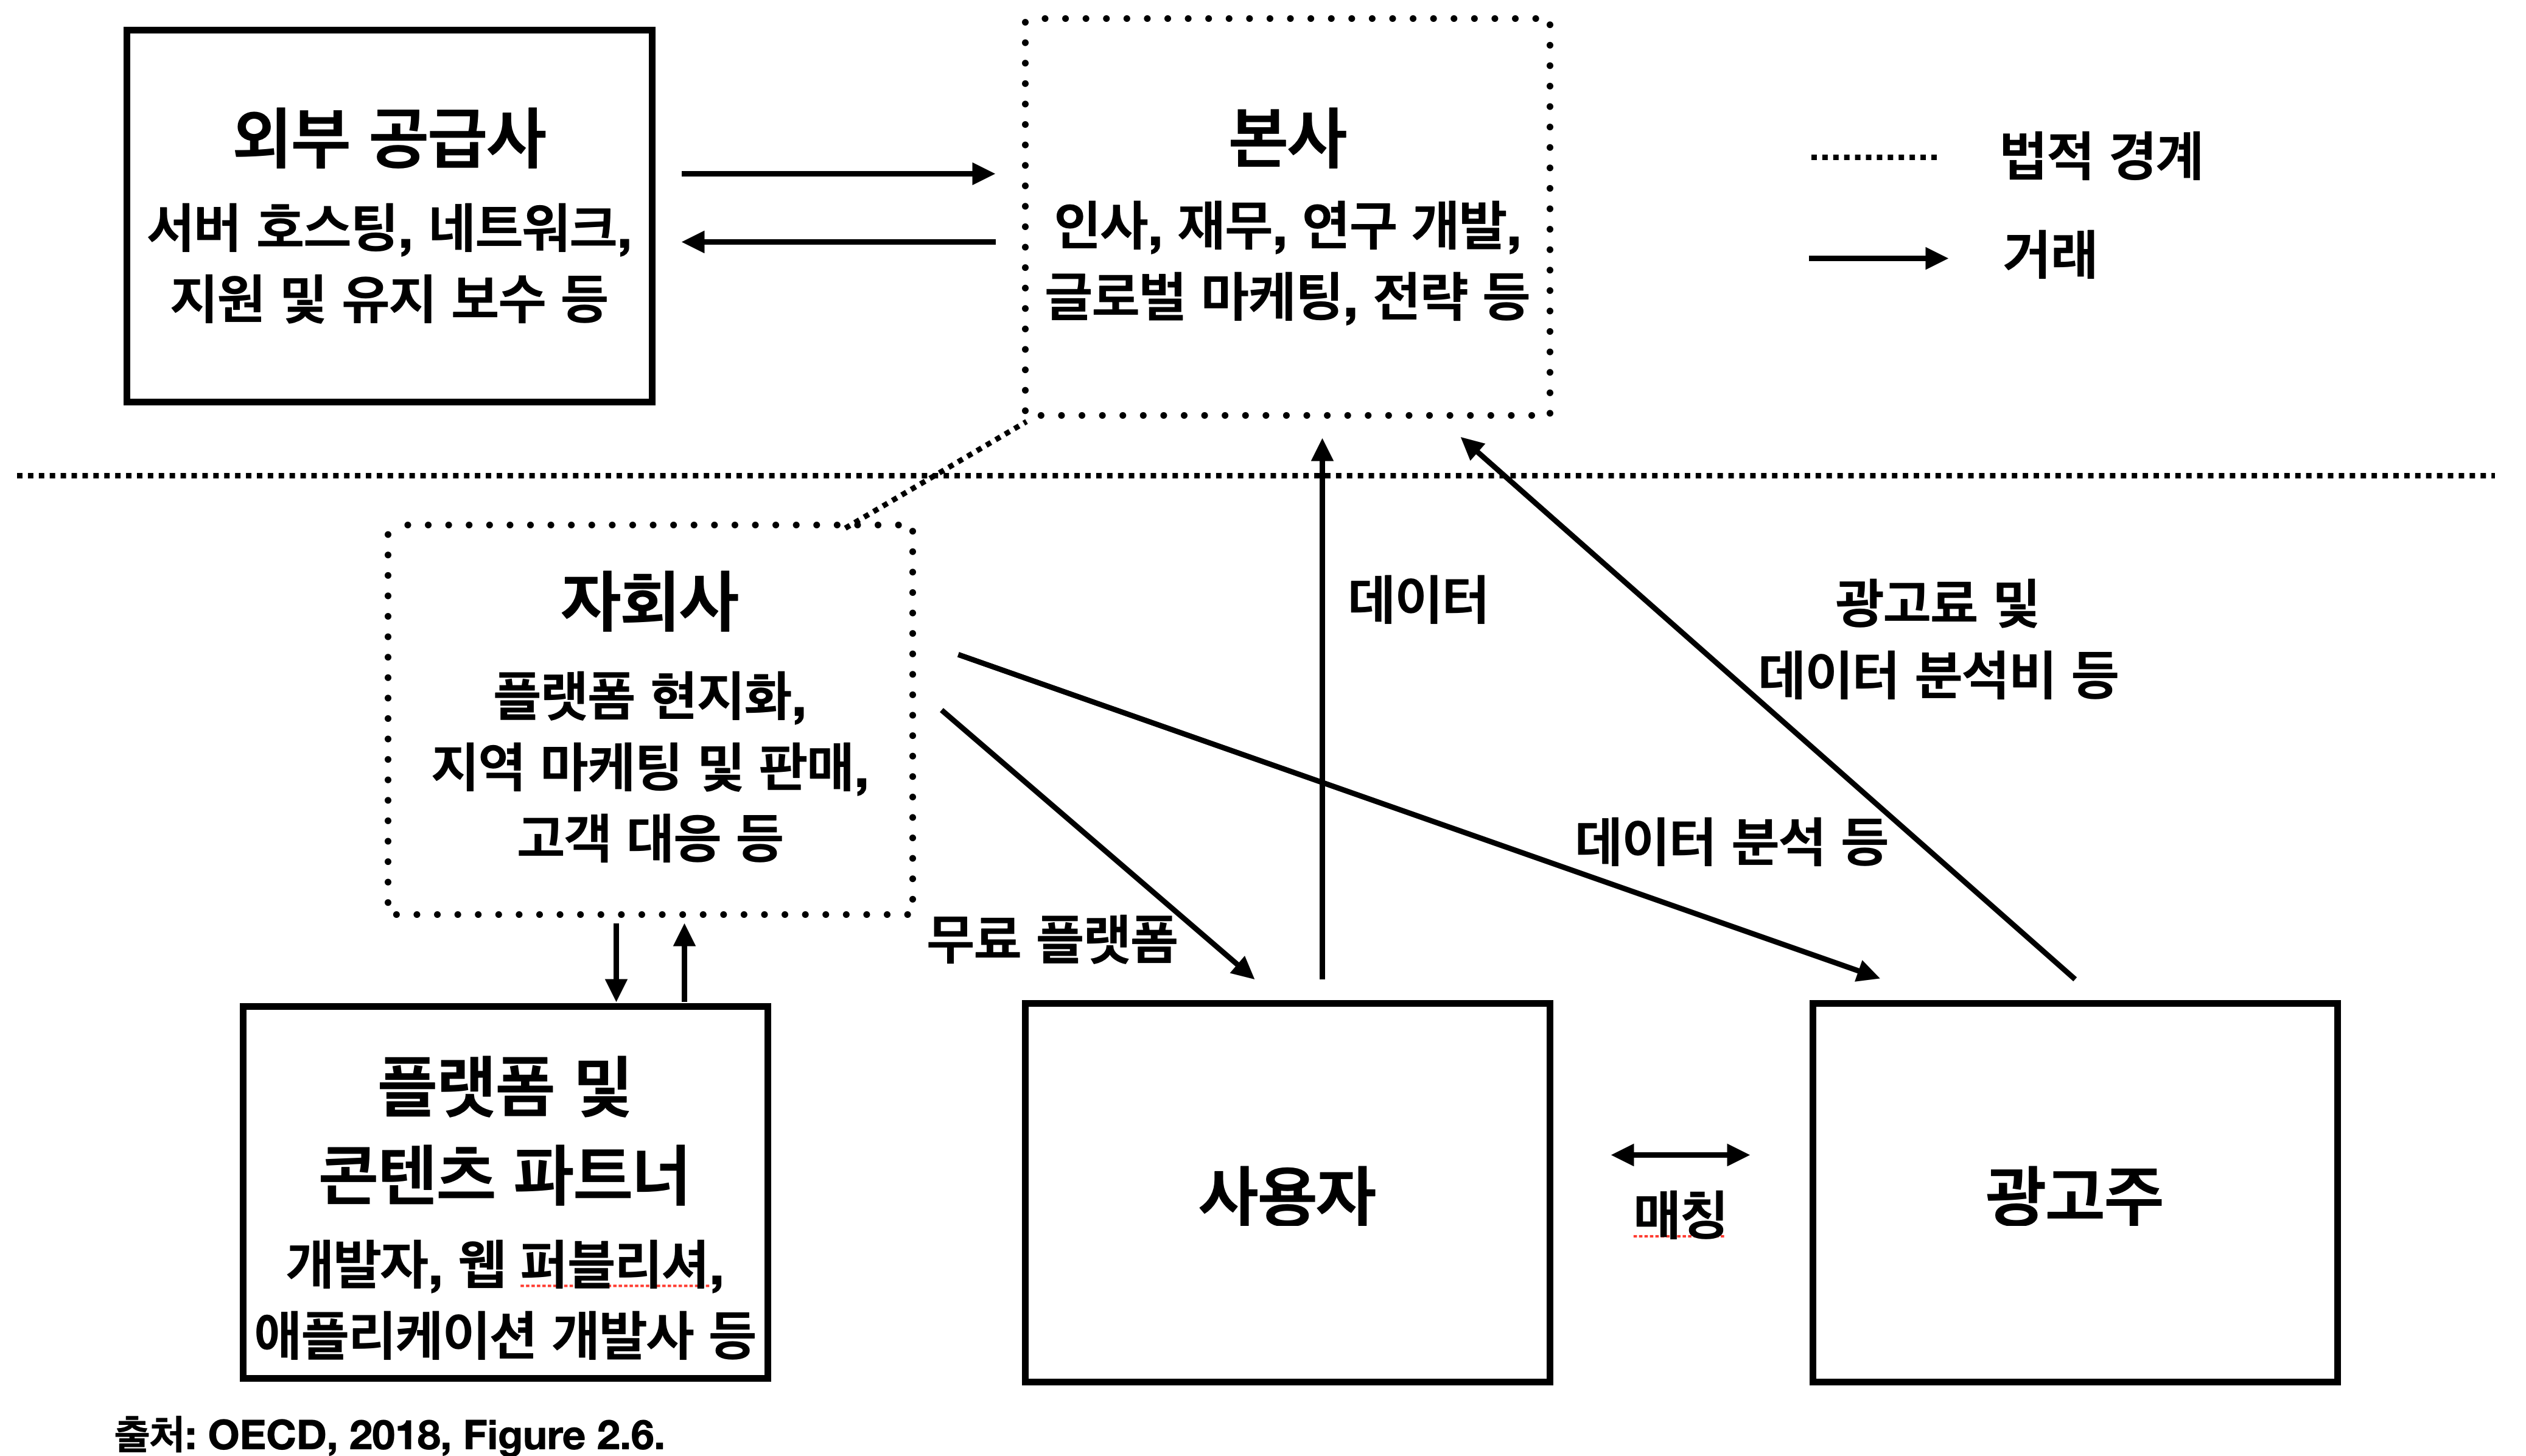
\includegraphics[scale=0.15]{schema.png}
				\caption{광고 기반 플랫폼 사업의 운영 개념도}
				\label{fig:schema}
				\end{center}
				\end{figure}		
			
		\item 또한, 광고 기반 플랫폼 사업의 경우, 광고주가 외국 기업이고, 외국 기업이 국내에 고정사업장을 두지 않은 플랫폼 사업자에게 지급하는 대가를 국내 원천 소득으로 볼 수 있는 근거가 조세 조약 및 국내세 법에 명시되어 있지 않음
		\item 다른 한 편, 플랫폼 사용자가 플랫폼에 개인 데이터를 대가로 지불한다고 보면, 개인의 거주지 국가가 이에 대해 과세권을 행사할 수 있다는 주장도 있음
		\end{itemize}
	\item 정상거래원칙(arm's length principle)에 근거한 무형 자산(지적재산권 등)에 대한 과세
				\begin{figure}[htbp]
				\begin{center}
				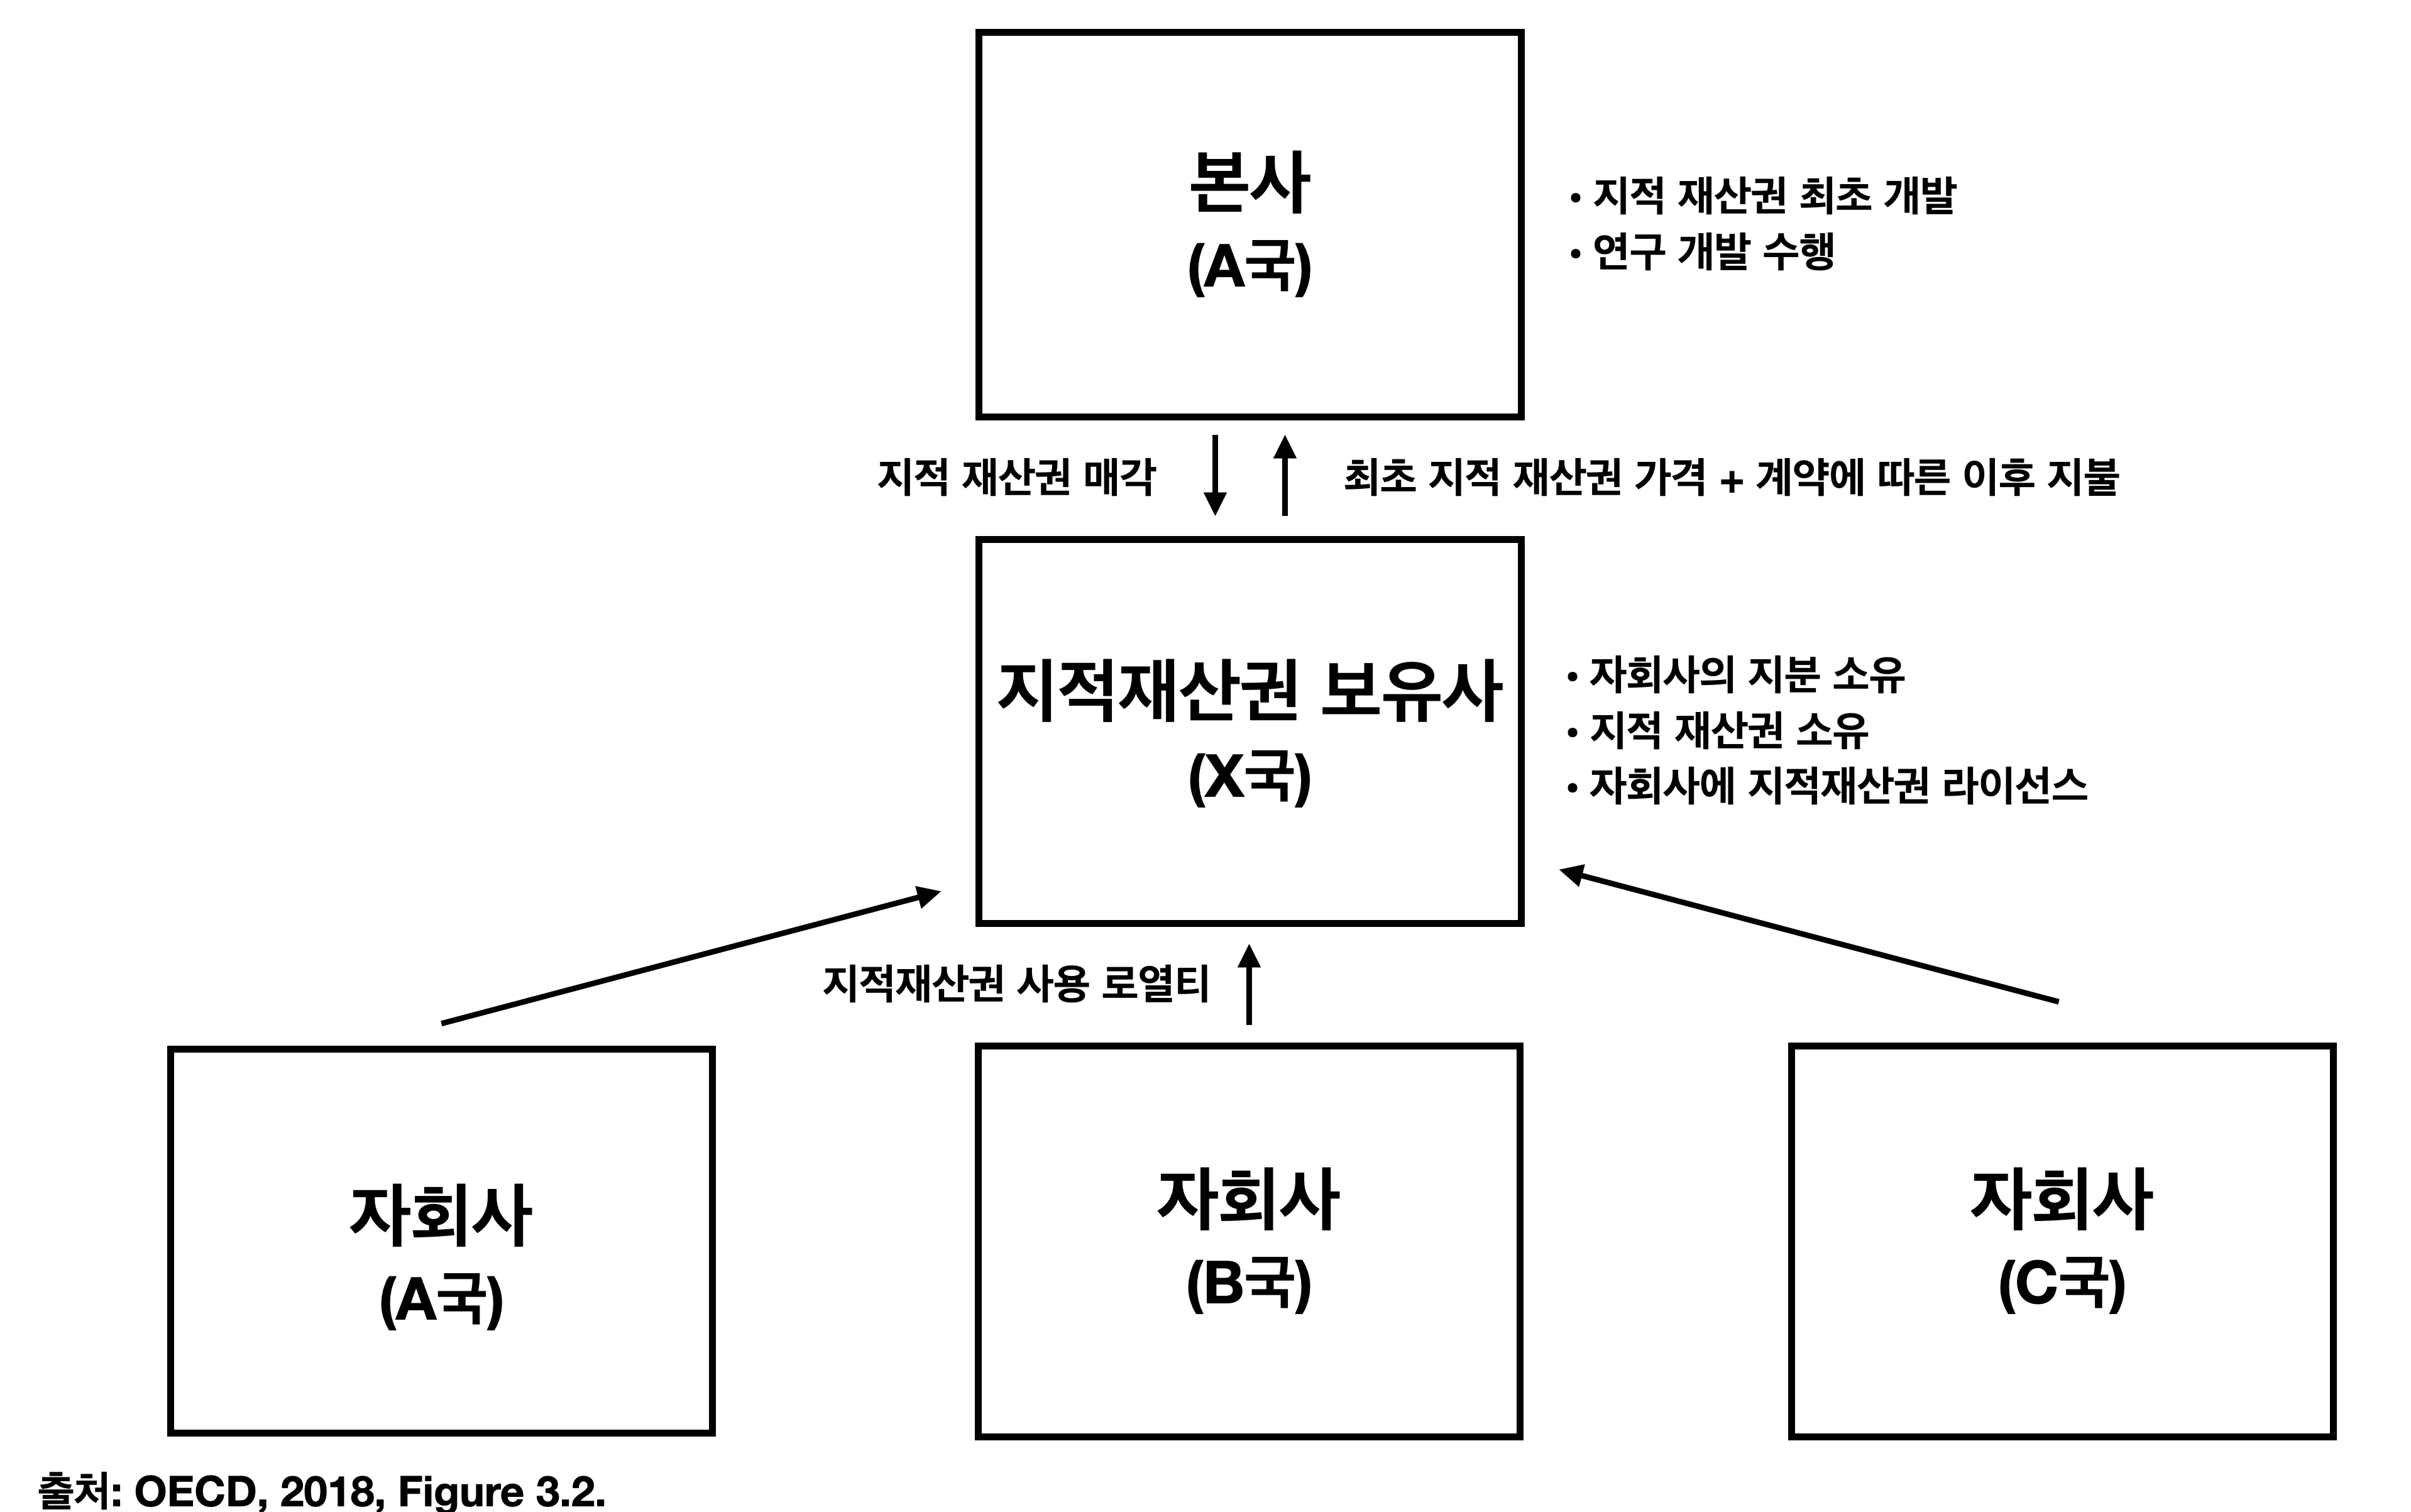
\includegraphics[scale=0.15]{schema2.png}
				\caption{로열티 수입 기업의 운영 개념도}
				\label{fig:schema}
				\end{center}
				\end{figure}	
		\begin{itemize}
		\item 국제적 조세 회피 $\rightarrow$ 즉, 소득 발생지 국가에 최소한의 사업 기능과 자산 및 위험만 두고, 그 외는 저세율 국가에 설립한 계열 회사로 이전하여, 계열 회사에 전세계에서 발생하는 소득을 유보시킴
			\begin{itemize}
			\item $\rightarrow$ 소득 발생지 국가의 세원 잠식, 과세소득의 해외 이전 발생
			\end{itemize}
		\item 혼성금융상품이나 혼성사업체를 이용한 국제적 이중 비과세 기법을 사용해 소득 발생지 국가에서의 세율을 낮추고 소득을 저세율 국가로 이전시키는 기법도 있음	
		\item 본사(A국)에서 지적재산권을 개발하고, 이를 조세율이 낮은 국가(X국)에 설립한 기업으로 이전하는 등, 이자, 배당, 사용료, 유가증권 양도소득 등에 대한 조약을 활용하여 조세 조약 상 소득 발생지 국가에서 원천징수를 할 수 없도록 되어 있는 국가에 회사를 설립하고 소득이 이 회사로 유입되도록 거래 구조를 변경
		\end{itemize}	
	\item 부가가치세(VAT: value added tax)의 국가간 형평성 저해
		\begin{itemize}
		\item 디지털 플랫폼 사업자가 소비자에게 원격으로 서비스를 공급하는 경우, 해외 공급자는 국내에서의 부가가치세를 부담하지 않을 수 있음
		\item 우리나라의 경우, 2015년 7월 이후 국내 사업장이 없는 외국 법인이 국내에 전자 서비스를 제공하는 경우 외국법인에 부가가치세를 과세할 수 있도록 함
		\end{itemize}	
	\end{itemize}
\end{itemize}

\section{디지털세 도입 논의}\label{sec:}
\begin{itemize}
\item 2012년 6월 G20 정상회담 및 재무장관 회의 이후 다국적 기업의 조세회피를 해결하기 위한 국제적 공동 대응이 주요 의제가 됨\footnote{이 절의 내용은 \cite{gimbichmalo-igyeong-geun:2019aa}, \cite{OECD/G20-Base-Erosion-and-Profit-Shifting-Project:2021uo}, \cite{yesangjun-otaehyeon:2021aa} 참고}
\item 2013년 OECD/G20 BEPS 프로젝트(Base Erosion and Profit Shifting Project)로 발전
	\begin{itemize}
	\item 2016년 2월 이후, OECD/G20 국가 외에도 전세계 140개국 참여
	\end{itemize} 
\item 2015년 11월 OECD/G20 BEPS 행동 계획 (BEPS Action Plan) 발표
	\begin{itemize}
	\item 디지털 경제에서의 조세 문제에 대한 특별한 권고 사항이 없었음
	\item $\rightarrow$ 주요 대상 기업이 누락됨에 따라 국제적 논의가 더 이상 진척되지 못함
	\end{itemize}
\item 2017년 3월, G20 재무장관 회의, 독일 주도로 	2018년까지 OECD/G20 BEPS 중간보고서 발간 결정
	\begin{itemize}
	\item 미국의 거대 기술 플랫폼 기업에 대한 유럽의 대응 논의
	\item 2017년 9월, 프랑스, 독일, 이탈리아, 스페인 등을 중심으로 균등세를 도입하자는 공동성명 발표
	\end{itemize}
\item 2018년 EU 집행위원회는 EU 차원의 디지털 세 입법을 추진
	\begin{itemize}
	\item $\rightarrow$ 회원국 간 의견 차이로 합의 실패	
	\item $\rightarrow$ 프랑스, 이탈리아, 스페인, 헝가리, 영국은 EU와 별도로 다음의 세 가지 입장에서 디지털 세 도입
		\begin{itemize}
		\item 새로운 고정사업장 개념을 적용
		\item 디지털 관련 소득을 원천 징수 대상 소득으로 분류
		\item 매출에 대한 과세
		\end{itemize}
	\item $\rightarrow$ 2019년 미국은 이들 국가의 디지털 서비스세 도입이 미국 기업에 대한 불공정 관행에 해당한다고 판단하고 보복관세 부과를 결정
	\end{itemize}
\item 2021년 미국이 적극적으로 BEPS 논의에 참여하며, 국제 디지털 세 도입이 빠르게 진행
	\begin{itemize}
	\item 2021년 3월 31일, 미국 바이든 대통령이 2조 2,500억 달러 규모의 인프라 투자 계획(American Jobs Plan)을 발표하고, 재원 마련을 위해 글로벌 최저한세 도입을 선언
	\item 2021년 6월 4-5일,  G7 재무장관/중앙은행 총재 회의에서 주요 원칙에 대한 합의가 이루어짐
		\begin{itemize}
		\item 2021년 7월 1일, OECD/G20 IF (Inclusive Framework) 총회에서 140개국 중 134개국이 6월의 회의와 합치된 합의안을 도출
			\begin{itemize}
			\item 8월 31일까지 비동의 6개국: 에스토니아, 헝가리, 아일랜드, 케냐, 나이지리아, 스리랑카
			\end{itemize}
		\end{itemize}
	\end{itemize}
\item 2021년 10월까지, 구체적인 실행 계획과 해결되지 않은 이슈에 대한 결론을 도출하기로 함
	\begin{itemize}
	\item 적용대상 기업, 배분량 구체화, 사업구분 기준 구체화, 이중과세 제거, 의무 불이행 시 대응 방안, 저세율국 최종모회사에 대한 비용 공제 부인 규칙 적용 시 추가 세액 상한 적용 여부, 최저한세율에 대한 최종 합의, 적용 예외 대상이 되는 초기 발전 단계의 다국적 기업에 대한 기준 등
	\item 나이지리아, 스리랑카, 케냐는 개발도상국에 대한 배려 조항으로 합의를 도출할 수 있을 것으로 전망
	\item 저세율국가(에스토니아, 헝가리, 아일랜드)의 반발
	\end{itemize}	
\item 2021년 10월 8일 \citep{OECD/G20-Base-Erosion-and-Profit-Shifting-Project:2021aa}	
	\begin{itemize}
	\item 136개국의 합의 발표
		\begin{itemize}
		\item 헝가리: 자동차 공장 등 자국 내 유형 자산에 대한 저세율을 향후 10년 간 유지 가능하도록, 장기 전환 기간을 인정 받음
		\item 아일랜드: 최저한세율이 최소 15\% 이상(at least)이라는 문구를 15\%로 조정
		\item 미합의:  나이지리아, 스리랑카, 케냐, 파키스탄
		\item 22년 국내 비준 및 국내법 개정, 23년 발효 및 시행	
		\end{itemize}
	\item 기둥 1 (Pillar I) 
		\begin{itemize}
		\item 목적: 고정사업장이 없더라도 시장에서 발생하는 매출을 기준으로 과세권을 부여
		\item 업종과 상관없이 매출액과 이익률 기준 상위 다국적 기업의 초과 이익에 대해 과세할 권리(Amount A)를 매출이 발생한 시장 소재국에 배분 
			\begin{itemize}
			\item 상위 다국적 기업: 글로벌 연결매출액 200억 유로 및 이익률 10\% 이상
			\item 이익률 $=$ 글로벌 세전 이익 / 글로벌 매출액
			\item 매출액 기준은 시행 7년 후 100억 유로로 축소
			\item 채굴업, 규제된 금융업 적용 제외
			\end{itemize}
		\item 과세연계점: 해당 사법권 내(국가 내)의 수입이 100만 유로 이상 발생할 경우
			\begin{itemize}
			\item 국내총생산이 400억 유로 이하인 국가의 경우 25만 유로 이상
			\end{itemize} 
		\item 초과이익 배분 비율 25\%로 합의
			\begin{itemize}
			\item Amount A $ = $ 매출액 $\times$ (세전 이익률 - 통상 이익률) $\times$ 25\%
			\end{itemize}
		\item 매출 귀속 기준: 재화나 서비스의 최종 거래가 발생하는 시장의 소재지에서 매출이 발생했다고 간주
		\item 과세 표준: 회계 기반, 손실은 이월, 구분 회계는 예외적인 경우에 한정하여 수행	
		\item 모든 분쟁 이슈는 의무적, 강제적 분쟁 해결 절차로 조정
			\begin{itemize}
			\item 단,  분쟁 대응역량이 낮은 개발도상국에 대해서는 강제적 분쟁 해결절차를 선택적으로 적용하고, 그 대상이 되는 지는 주기적으로 재심사
			\end{itemize}
		\item 기존의 디지털 서비스 세 및 관련 유사 조치는 폐지하며 향후에도 도입하지 않음
		\item 2022년까지 실행을 위한 다자 협약을 발전시키고 2023년 발효를 목표로 함
		\end{itemize}
	\item 기둥 2 (Pillar II) 
		\begin{itemize}
		\item 목적: 글로벌 최저한세를 통해 국가 간 조세 경쟁을 막음
		\item 대상: 글로벌 (연결)매출액이 7억 5,000만 유로를 넘는 다국적 기업
			\begin{itemize}
			\item 다국적 기업의 본사 소재국은 매출액 기준과 무관하게 적용
			\item 국제 해운업 제외: 실제 이익이 아닌 선박의 순톤수와 운항 일수를 기준으로 과세 표준 산출하는 톤세 제도 적용
			\end{itemize}
		\item GloBE (Global Anti-Base Erosion Proposal) 규칙: 소득산입규칙과 비용공제부인규칙으로 구성 $\rightarrow$ 도입 국가의 국내법
			\begin{itemize}
			\item 소득 산입 규칙: 자회사의 소득이 저율로 과세되는 경우, 소득산입규칙을 갖고 있는 최종모회사 소재국에 우선적으로 납부 의무가 발생하며, 해당 법인이 제3자와 지분을 분할 소유하면(80\% 미만), 차상위 중간모회사에 소득산입규칙을 대신 적용
			\item 비용 공제 부인 규칙: 소득산입규칙에 따라 초과 세액이 배분되지 않는 경우, 저세율국(최종 모회사 소재지 포함) 구성회사에 지급금을 지불한 법인이 최저한세율과의 차이만큼 추가세액을 납부
			\item 해외 진출 초기 단계의 다국적 기업은 비용 공제 부인 규칙을 5년간 적용 예외
			\item 비용공제부인규칙 발효 시점을 2024년으로 유예
			\item 소득산입규칙과 비용공제부인규칙에 적용되는 최저한세율: 15\%
			\item GloBE 규칙의 도입은 국가별 재량에 따르나 도입 시, 합의된 규칙과 일치해야 하며, 다른 회원국이 규칙을 실행하면 모든 회원국이 이를 받아들여야 함	
			\end{itemize}
		\item 원천지 국 과세 규칙  $\rightarrow$ 양자간 조세 조약
			\begin{itemize}
			\item 저세율국 소재 국외 관계사의 이자, 사용료 등 지급금에 대해 최저한세율 9\% 보다 낮은 명목 세율 적용 시, 양자간 조세 조약에 기반하여 원천지 국에 추가 과세권 인정
			\end{itemize}
		\item 2022년까지 회원국의 관련 법 개정 후, 2023년 발효	
		\end{itemize}
	\end{itemize}
\end{itemize}

\pagebreak

\section*{정리하기}
\begin{enumerate}
\item 디지털 경제의 사업 유형은 다면 플랫폼, 재판매, 수직통합, 중간재 공급 등으로 나눌 수 있다.
\item 플랫폼 사업과 디지털화로 인해, 소득의 원천이 되는 국가에 물리적 고정사업장을 두지 않고 사법 경계를 가로질러 대단위 경제 활동이 가능해졌다. 또 소프트웨어와 알고리듬 등의 무형 재산과 데이터, 사용자 참여는 시너지 효과를 내며 사용자가 부가가치를 만들고 있다.
\item 고정사업장이 없는 경제 활동은 고정사업장 소재지국의 과세권 행사라는 원칙을 위협한다.
\item 다국적 기업은 저세율 국가에 설립한 계열 회사로 무형자산에 대한 권리를 이전시켜, 전세계적 차원의 조세 회피가 가능하다.
\item 2012년부터 다국적 기업의 조세 회피에 대한 국제적 공동 대응이 본격적으로 논의되었으며 2021년 10월 전세계 136개국이 국제 디지털세 도입에 합의하게 되었다.
\item 국제 디지털 세는 크게 두 개의 기둥으로 이루어져있으며, 하나는 고정사업장이 없더라도 시장에서 발생하는 매출을 기준으로 매출이 발생한 국가가 과세권을 갖는 것이다. 다른 하나는 글로벌 최저한세율 15\%를 도입하여 국가 간 조세 경쟁을 막는 것이다.
\item 2021년의 합의는 2022년 국가 별 비준 및 세부 협약을 발전시키고 2023년 발효를 목표로 하고 있다.
\end{enumerate}